
\chapter{The Issue Unit}

The issue window holds dispatched micro-ops that have not yet executed.  When all of the operands for the micro-op are ready, the issue slot sets its ``request" bit high.  The issue select logic then chooses to issue a slot which is asserting its ``request" signal.  Once a micro-op is issued, it is removed from the issue window to make room for more dispatched instructions. 

Future designs may choose to *speculatively* issue micro-ops (e.g., speculating that a load instruction will hit in the cache and thus issuing dependent micro-ops assuming the load data will be available in the bypass network). In such a scenario, the issue window cannot remove speculatively issued micro-ops until the speculation has been resolved. If a speculatively-issued micro-op failure occurs, 



\section{Issue Slot}

Figure \ref{fig:riscv-boom_issue_slot} shows a single issue slot from the {\em Issue Window}.\footnote{Conceptually, a bus is shown for implementing the driving of the signals sent to the {\em Register Read} Stage.  In reality BOOM actually uses muxes.}

Instructions (actually they are ``micro-ops" by this stage) are {\em dispatched} into the {\em Issue Window}.  From here, they wait for all of their operands to be ready (``p" stands for {\em presence} bit, which marks when an operand is {\em present} in the register file).  

Once ready, the {\em issue slot} will assert its ``request" signal, and wait to be {\em issued}.  Currently, BOOM only issues a single micro-op every cycle, and has a fixed priority encoding to give the lower ID entries priority.


\begin{figure}[ht]
	\centering
	\centerline{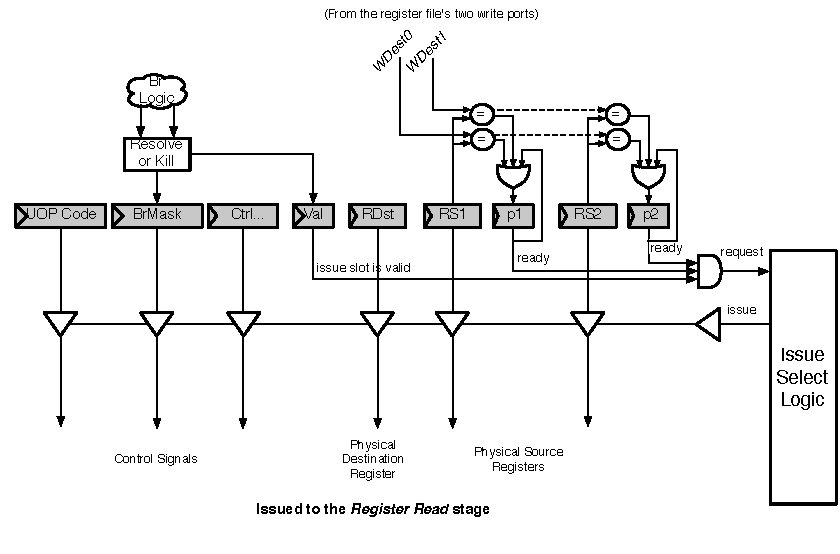
\includegraphics[scale =1.0] {figures/issue_slot}}
	\caption{ \small A single issue slot from the Issue Window.}
	\label{fig:riscv-boom_issue_slot}
\end{figure}

\section{Issue Select Logic}



\section{Un-ordered Issue Window}

\section{Age-ordered Issue Window}
